\section{Was erkannt werden soll}
Im Gegensatz zu herkömmlichen Beschreibungen von Mechanismen durch Glieder und Gelenke modelliert \name{mec2} Mechanismen durch \name{Nodes} und \name{Constraints} \cite{Goessner2019a}.
Beispielhaft zeigt Abbildung \ref{fig:4bar} ein Viergelenk mit der zugehörigen Beschreibung des Mechanismus im JSON-Format.

\begin{figure}
  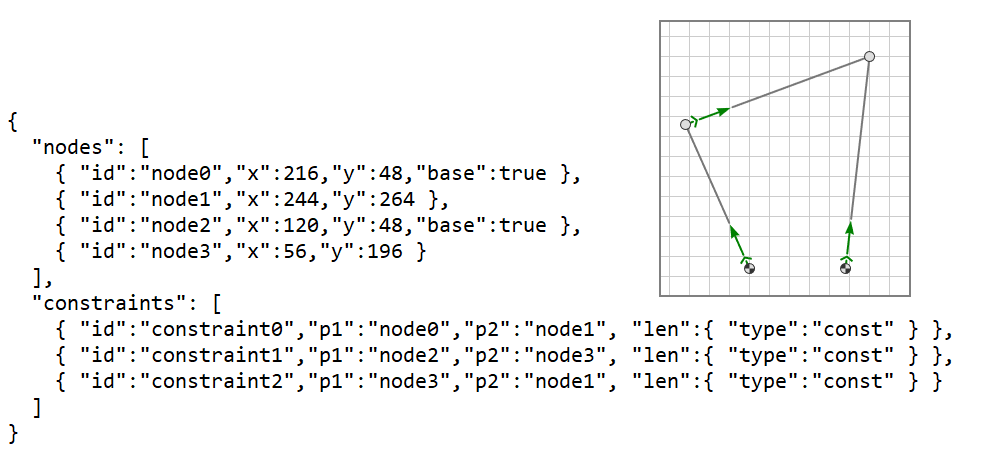
\includegraphics[width=\textwidth]{images/4bar_json}
  \caption{Die JSON-Darstellung eines durch mec2 erstellten Viergelenks mit dem entsprechend generierten Mechanismus.}
  \label{fig:4bar}
\end{figure}

Um solche Mechanismen durch Handzeichnungen zu erstellen, ist es erforderlich, einen Algorithmus zu trainieren, der mit einer entsprechenden Skizze als Input solchen JSON-Code als Output produziert.

Hierfür werden zunächst Trainingsdaten geschaffen, anhand derer ein trainierbarer Algorithmus Merkmale erlernen und so Eingangsbilder den entsprechenden Lösungen zuordnen kann.
Für dieses Projekt wurden etwa 1200 Nodes, 1200 Base-Nodes und 1200 nicht zutreffende Bilder erstellt.
Diese wurden vor dem Training durch Rotation und Spiegelung augmentiert, um die Varianz der Trainingsdaten zu erhöhen.

Dem zu trainierendem Algorithmus wurde zusätzlich beigebracht, die von \name{mec2} genutzten Symbole den nicht zutreffenden Bildern zuzuordnen.
Damit wird erreicht, dass Mechanismen erweitert werden können, ohne die bereits erkannten Elemente wiederholt zu erkennen.

\begin{figure}
  \centering
    \begin{subfigure}[b]{0.4\textwidth}
        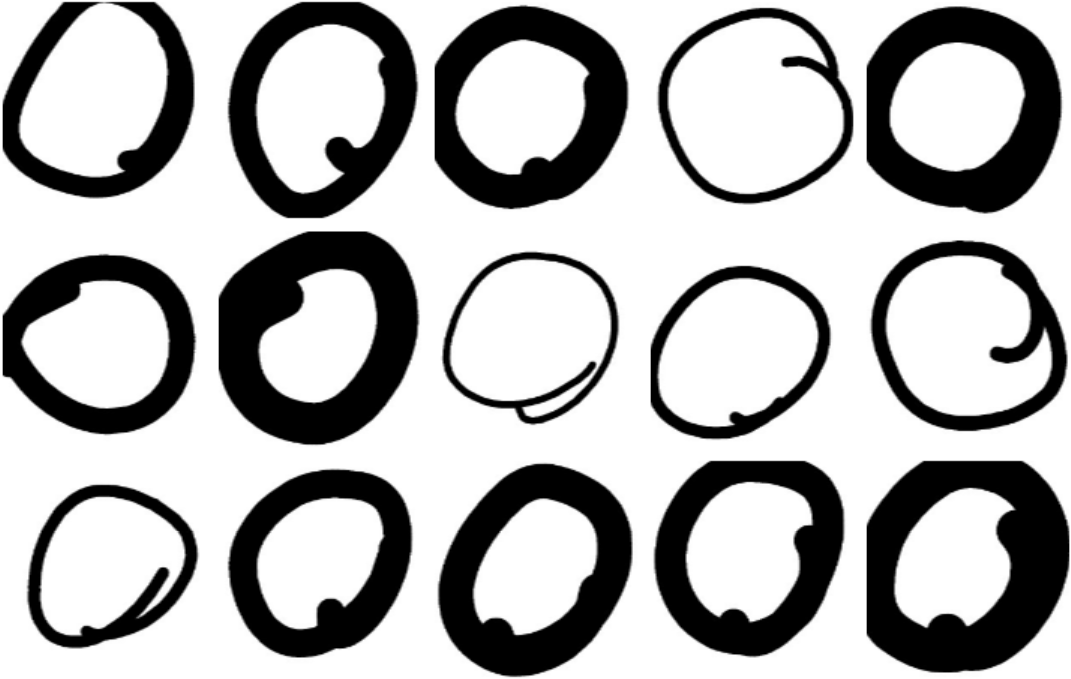
\includegraphics[width=\textwidth]{images/os.png}
        \caption{Nodes}
        \label{fig:os}
    \end{subfigure}
    \begin{subfigure}[b]{0.4\textwidth}
        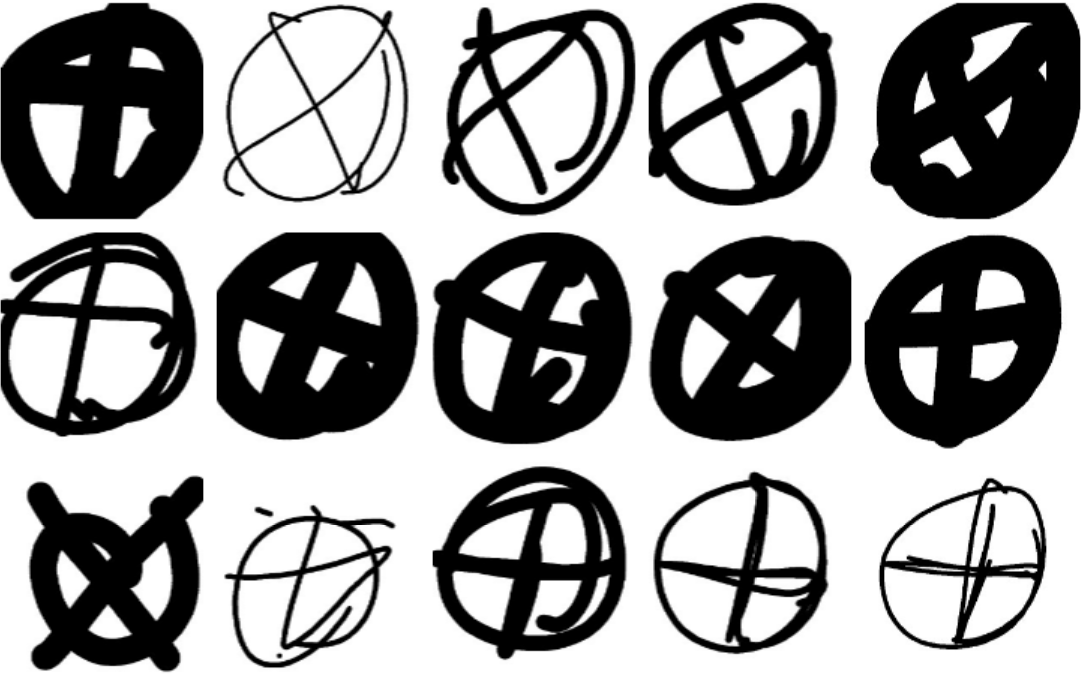
\includegraphics[width=\textwidth]{images/xs.png}
        \caption{Base-Nodes}
        \label{fig:xs}
    \end{subfigure}
    \begin{subfigure}[b]{0.4\textwidth}
      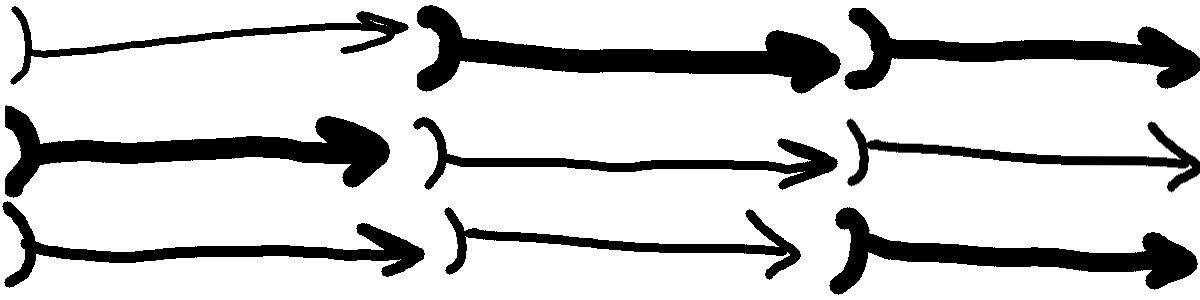
\includegraphics[width=\textwidth]{images/rs.png}
      \caption{rotatorische Constraints}
      \label{fig:rs}
    \end{subfigure}
    \begin{subfigure}[b]{0.4\textwidth}
      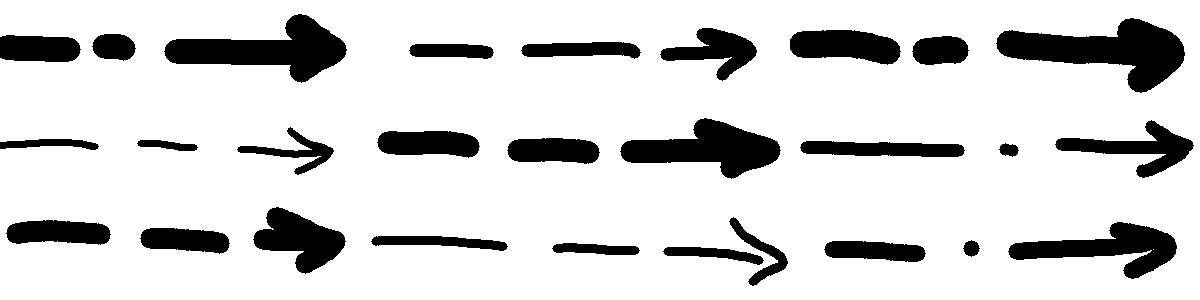
\includegraphics[width=\textwidth]{images/ts.png}
      \caption{translatorische Constraints}
      \label{fig:ts}
    \end{subfigure}
    \caption{Beispiele für handgezeichnete Symbole welche zum Trainieren der Algorithmen genutzt werden.}
    \label{fig:example_symbols}
\end{figure}

Neben den Nodes wurden für die Constraints wieder 1200 rotatorische und 1200 translatorische Verbindungen gezeichnet.
Sie orientieren sich in ihrer Gestaltung an der Darstellung von Constraints in Abbildung \ref{fig:constraints_gtk}.
Zum aktuellen Stand des Projekts sind gebundene und freie Constraints nicht implementiert.

\begin{figure}
  \centering
  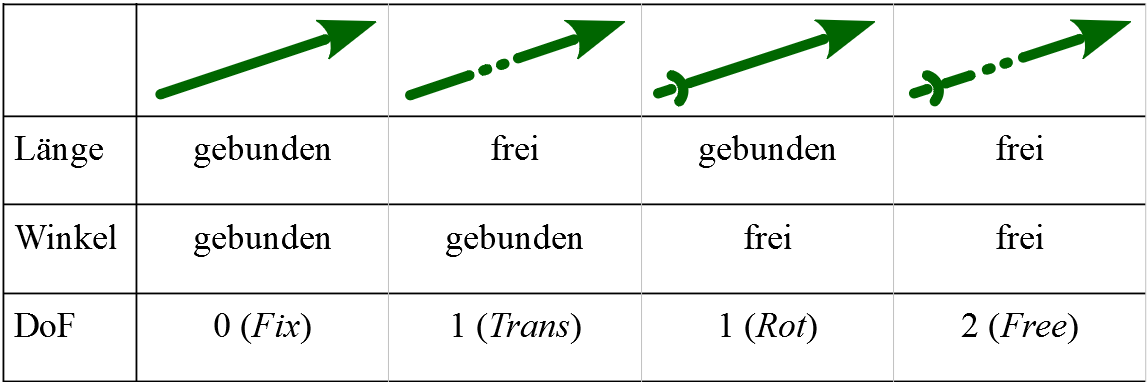
\includegraphics[width=0.8\textwidth]{images/gtk2019_tab1.png}
  \caption{Darstellung der Constraints in ihren vier Ausprägungen. \cite[Tab. 1]{Goessner2019a}}.
  \label{fig:constraints_gtk}
\end{figure}
